% Options for packages loaded elsewhere
\PassOptionsToPackage{unicode}{hyperref}
\PassOptionsToPackage{hyphens}{url}
\PassOptionsToPackage{dvipsnames,svgnames,x11names}{xcolor}
%
\documentclass[
  11pt,
  letterpaper,
]{article}

\usepackage{amsmath,amssymb}
\usepackage{iftex}
\ifPDFTeX
  \usepackage[T1]{fontenc}
  \usepackage[utf8]{inputenc}
  \usepackage{textcomp} % provide euro and other symbols
\else % if luatex or xetex
  \usepackage{unicode-math}
  \defaultfontfeatures{Scale=MatchLowercase}
  \defaultfontfeatures[\rmfamily]{Ligatures=TeX,Scale=1}
\fi
\usepackage{lmodern}
\ifPDFTeX\else  
    % xetex/luatex font selection
\fi
% Use upquote if available, for straight quotes in verbatim environments
\IfFileExists{upquote.sty}{\usepackage{upquote}}{}
\IfFileExists{microtype.sty}{% use microtype if available
  \usepackage[]{microtype}
  \UseMicrotypeSet[protrusion]{basicmath} % disable protrusion for tt fonts
}{}
\makeatletter
\@ifundefined{KOMAClassName}{% if non-KOMA class
  \IfFileExists{parskip.sty}{%
    \usepackage{parskip}
  }{% else
    \setlength{\parindent}{0pt}
    \setlength{\parskip}{6pt plus 2pt minus 1pt}}
}{% if KOMA class
  \KOMAoptions{parskip=half}}
\makeatother
\usepackage{xcolor}
\usepackage[margin=1in]{geometry}
\setlength{\emergencystretch}{3em} % prevent overfull lines
\setcounter{secnumdepth}{-\maxdimen} % remove section numbering
% Make \paragraph and \subparagraph free-standing
\ifx\paragraph\undefined\else
  \let\oldparagraph\paragraph
  \renewcommand{\paragraph}[1]{\oldparagraph{#1}\mbox{}}
\fi
\ifx\subparagraph\undefined\else
  \let\oldsubparagraph\subparagraph
  \renewcommand{\subparagraph}[1]{\oldsubparagraph{#1}\mbox{}}
\fi


\providecommand{\tightlist}{%
  \setlength{\itemsep}{0pt}\setlength{\parskip}{0pt}}\usepackage{longtable,booktabs,array}
\usepackage{calc} % for calculating minipage widths
% Correct order of tables after \paragraph or \subparagraph
\usepackage{etoolbox}
\makeatletter
\patchcmd\longtable{\par}{\if@noskipsec\mbox{}\fi\par}{}{}
\makeatother
% Allow footnotes in longtable head/foot
\IfFileExists{footnotehyper.sty}{\usepackage{footnotehyper}}{\usepackage{footnote}}
\makesavenoteenv{longtable}
\usepackage{graphicx}
\makeatletter
\def\maxwidth{\ifdim\Gin@nat@width>\linewidth\linewidth\else\Gin@nat@width\fi}
\def\maxheight{\ifdim\Gin@nat@height>\textheight\textheight\else\Gin@nat@height\fi}
\makeatother
% Scale images if necessary, so that they will not overflow the page
% margins by default, and it is still possible to overwrite the defaults
% using explicit options in \includegraphics[width, height, ...]{}
\setkeys{Gin}{width=\maxwidth,height=\maxheight,keepaspectratio}
% Set default figure placement to htbp
\makeatletter
\def\fps@figure{htbp}
\makeatother
\newlength{\cslhangindent}
\setlength{\cslhangindent}{1.5em}
\newlength{\csllabelwidth}
\setlength{\csllabelwidth}{3em}
\newlength{\cslentryspacingunit} % times entry-spacing
\setlength{\cslentryspacingunit}{\parskip}
\newenvironment{CSLReferences}[2] % #1 hanging-ident, #2 entry spacing
 {% don't indent paragraphs
  \setlength{\parindent}{0pt}
  % turn on hanging indent if param 1 is 1
  \ifodd #1
  \let\oldpar\par
  \def\par{\hangindent=\cslhangindent\oldpar}
  \fi
  % set entry spacing
  \setlength{\parskip}{#2\cslentryspacingunit}
 }%
 {}
\usepackage{calc}
\newcommand{\CSLBlock}[1]{#1\hfill\break}
\newcommand{\CSLLeftMargin}[1]{\parbox[t]{\csllabelwidth}{#1}}
\newcommand{\CSLRightInline}[1]{\parbox[t]{\linewidth - \csllabelwidth}{#1}\break}
\newcommand{\CSLIndent}[1]{\hspace{\cslhangindent}#1}

\usepackage{amsfonts}
\DeclareMathAlphabet{\mathams}{U}{msb}{m}{n}
\usepackage{booktabs}
\usepackage{longtable}
\usepackage{array}
\usepackage{multirow}
\usepackage{wrapfig}
\usepackage{float}
\usepackage{colortbl}
\usepackage{pdflscape}
\usepackage{tabu}
\usepackage{threeparttable}
\usepackage{threeparttablex}
\usepackage[normalem]{ulem}
\usepackage{makecell}
\usepackage{xcolor}
\makeatletter
\makeatother
\makeatletter
\makeatother
\makeatletter
\@ifpackageloaded{caption}{}{\usepackage{caption}}
\AtBeginDocument{%
\ifdefined\contentsname
  \renewcommand*\contentsname{Table of contents}
\else
  \newcommand\contentsname{Table of contents}
\fi
\ifdefined\listfigurename
  \renewcommand*\listfigurename{List of Figures}
\else
  \newcommand\listfigurename{List of Figures}
\fi
\ifdefined\listtablename
  \renewcommand*\listtablename{List of Tables}
\else
  \newcommand\listtablename{List of Tables}
\fi
\ifdefined\figurename
  \renewcommand*\figurename{Figure}
\else
  \newcommand\figurename{Figure}
\fi
\ifdefined\tablename
  \renewcommand*\tablename{Table}
\else
  \newcommand\tablename{Table}
\fi
}
\@ifpackageloaded{float}{}{\usepackage{float}}
\floatstyle{ruled}
\@ifundefined{c@chapter}{\newfloat{codelisting}{h}{lop}}{\newfloat{codelisting}{h}{lop}[chapter]}
\floatname{codelisting}{Listing}
\newcommand*\listoflistings{\listof{codelisting}{List of Listings}}
\makeatother
\makeatletter
\@ifpackageloaded{caption}{}{\usepackage{caption}}
\@ifpackageloaded{subcaption}{}{\usepackage{subcaption}}
\makeatother
\makeatletter
\@ifpackageloaded{tcolorbox}{}{\usepackage[skins,breakable]{tcolorbox}}
\makeatother
\makeatletter
\@ifundefined{shadecolor}{\definecolor{shadecolor}{rgb}{.97, .97, .97}}
\makeatother
\makeatletter
\makeatother
\makeatletter
\makeatother
\ifLuaTeX
  \usepackage{selnolig}  % disable illegal ligatures
\fi
\IfFileExists{bookmark.sty}{\usepackage{bookmark}}{\usepackage{hyperref}}
\IfFileExists{xurl.sty}{\usepackage{xurl}}{} % add URL line breaks if available
\urlstyle{same} % disable monospaced font for URLs
\hypersetup{
  pdftitle={Qualifying Exam},
  pdfauthor={Art Tay},
  colorlinks=true,
  linkcolor={blue},
  filecolor={Maroon},
  citecolor={Blue},
  urlcolor={Blue},
  pdfcreator={LaTeX via pandoc}}

\title{Qualifying Exam}
\author{Art Tay}
\date{}

\begin{document}
\maketitle
\ifdefined\Shaded\renewenvironment{Shaded}{\begin{tcolorbox}[frame hidden, breakable, interior hidden, sharp corners, borderline west={3pt}{0pt}{shadecolor}, enhanced, boxrule=0pt]}{\end{tcolorbox}}\fi

\hypertarget{introduction}{%
\section{Introduction}\label{introduction}}

\begin{itemize}
\item
  Overview of the problem area.

  \begin{itemize}
  \tightlist
  \item
    Graphs are an important data structure.

    \begin{itemize}
    \tightlist
    \item
      GRAPHS provide an incredibly flexible structure for modeling
      complex data. Data can naturally appear as graphs, like molecules.
      We can reduce data to a graph, such as the key points of a image.
      We can even use graphs to add structure, such as grammatical
      relationships.
    \end{itemize}
  \item
    GNN models are good at prediction and inference on graph data.

    \begin{itemize}
    \tightlist
    \item
      Graph Neural Networks (GNNs) have become a popular choice for
      prediction and inference on graph data. At their core, GNNs work
      by iteratively updating node embeddings based on information from
      neighboring nodes. The idea is to use the graph's structure to
      engineer better features. This message passing scheme allows GNNs
      to capture complex dependencies and patterns present within the
      graph structure. GNN architectures typically consist of multiple
      layers, each performing message passing and aggregation operations
      to refine the embeddings. These layers are often followed by
      pooling and dense prediction layers to produce the final output.
    \end{itemize}
  \item
    There are many important applications for graph classification
    models.

    \begin{itemize}
    \tightlist
    \item
      Some important applications of graph classification include
      predicting chemical toxicity (Bai et al. 2019), classifying
      proteins (Gallicchio and Micheli 2019), and even detecting cancer
      from pathology slides (Xiao et al. 2023).
    \end{itemize}
  \item
    \textbf{Problem:} While GNNs achieve remarkable predictive power,
    their complexity prevents the exaction of the scientific rationale.
  \end{itemize}
\item
  Why is the problem important?

  \begin{itemize}
  \tightlist
  \item
    Explaining or interpreting GNN predictions would

    \begin{itemize}
    \tightlist
    \item
      help with the adoption of such models for critical applications,
    \item
      prevent adversarial attacks,
    \item
      detect potential implicit discrimination,
    \item
      guide scientific as well as machine learning research.
    \end{itemize}
  \end{itemize}
\item
  How does the problem relate to the fundamentals areas of Statistics?

  \begin{itemize}
  \item
    Explain-ability vs Interpretability

    \begin{itemize}
    \tightlist
    \item
      Yuan et al. (2022)
    \item
      A model is interpretable if the models decision process can be
      readily understood by humans. For example, a linear regression
      model is interpretable because the coefficient clearly define how
      any prediction get made.
    \item
      A model is explainable if the models prediction can be reasoned
      post-hoc. Permuting each variable and measuring the variation in
      the predictions can be used to estimate each variables marginal
      effect {[}cite{]}.
    \end{itemize}
  \item
    One goal would be to create a GNN type model whose decision process
    is human interpretable. A straight translation from statistics would
    be a circuit type analysis {[}cite{]}. For graphs, this would mean
    some form of coefficients on subgraphs producing the prediction.
  \item
    Another goal might be to develope a method that determines if a
    feature is statistical significant to the GNN model. The challenge
    is that the graph features that matter to researchers aren't
    necessarily tabular.
  \end{itemize}
\item
  What is the impact of solving this problem?

  \begin{itemize}
  \item
    In the application where GNNs have shown strong predictive power, we
    can exact a testable scientific hypothesis for the nature of the
    classification.
  \item
    In the application where GNNs have weak predictive power, highlight
    the potential misunderstandings the model is having.
  \end{itemize}
\end{itemize}

\hypertarget{notation}{%
\section{Notation}\label{notation}}

\begin{itemize}
\item
  Let \(G\) denote a graph.
\item
  Any graph \(G\) can be describe by \(X, A, E\). The node feature
  matrix, edge feature matrix, and adjacency matrix respectively
\item
  Let \(X = [X_c, \ X_d]\), where \(X_c\) is the subset of continuous
  node features and \(X_d\) is the subset of one-hot discrete node
  features.
\item
  Let \(E = [E_c, \ E_d]\), denoted in the same manner.
\item
  Let \(n\) represent the number of nodes in the graph and \(v\)
  represent the number of edges.
\item
  Let \(\text{feat}_{(.)}\) denote the number of features or columns in
  the the corresponding feature matrix.
\item
  \(A\) is a binary \(n \times n\) matrix where \(A[i, \ j] = 1\)
  indicates that an edge exists between nodes labeled \(i\) and \(j\).
\item
  Let
  \(\text{explainee}(G; \ \Omega) = h^{(1)}_G, \dots h^{(L)}_G, \rho_G\)
  be an \(L\) layer GNN model with parameters \(\Omega\) that we would
  like to explain.
\item
  For any graph Let \(\nu\) denote the set of node and \(\mathcal{E}\)
  denote the set of edges.
\end{itemize}

\hypertarget{analysis-of-core-papers}{%
\section{Analysis of Core Papers}\label{analysis-of-core-papers}}

\hypertarget{gnninterpreter}{%
\subsection{GNNInterpreter}\label{gnninterpreter}}

(Wang and Shen 2024)

\begin{itemize}
\item
  Overview

  \begin{itemize}
  \item
    Instance v. Model Level

    \begin{itemize}
    \tightlist
    \item
      In general, explanation methods serve to elucidate which features
      within the data influence disparate predictions. These methods
      typically fall into two categories: instance-level and
      model-level. Instance-level explanations aim to unveil the model's
      rationale behind a particular prediction. In domains such as image
      and text analysis, a prevalent approach involves masking or
      perturbing the instance and assessing the impact on the model's
      prediction. On the other hand, model-level explanations seek to
      understand how a model generally distinguishes between classes. In
      image and text analysis, for instance, one common technique
      involves treating the input as a trainable parameter and
      optimizing the model's prediction towards a specific class.
      Consequently, the resulting optimized input comprises a set of
      features strongly associated with the targeted class.
    \end{itemize}
  \item
    GNNInterpreter provides model level explanations for GNN in this
    manner.
  \item
    Formally, GNNInterpreter tries to learn the graph generating
    distribution for each class.
  \item
    GNNInterpreter works by optimizing the parameters of a generic graph
    generating distribution to produce samples that closely match the
    explainee's understanding of the targeted class.
  \end{itemize}
\item
  Explanation of the graph generating distribution.

  \begin{itemize}
  \item
    Graph generating distributions are hard to specify because there can
    be discrete and continuous elements of \(X\), \(E\) and \(A\).
    Furthermore, the interactions between these matrices can be complex.
  \item
    The authors tackle these issues by making two simplify assumptions.

    \begin{enumerate}
    \def\labelenumi{\arabic{enumi}.}
    \item
      Assume that \(G\) is a \emph{Gilbert} random graph, every possible
      edge as an independent fixed probability of occurring.
      \begin{equation}
           \forall (i, \ j) \neq (k, l) \ Pr(A[i, \ j] = 1) \perp Pr(A[k, \ l] = 1)
       \end{equation}
    \item
      The features of every node and edge are independently distributed.
    \end{enumerate}
  \item
    The author justify these assumptions by:

    \begin{enumerate}
    \def\labelenumi{\arabic{enumi}.}
    \tightlist
    \item
      The other graph distributions aren't suitable.

      \begin{enumerate}
      \def\labelenumii{\alph{enumii}.}
      \tightlist
      \item
        Erdo-Renyi graphs have a fixed number of edges (and nodes, but
        nodes are also fixed for Gilbert).
      \item
        Rado graphs are infinite in size.
      \item
        The random dot-product graph model is just a generalization of
        Gilbert random graphs.
      \end{enumerate}
    \item
      Because the parameters of the independent distributions will be
      updated jointly using the \emph{explainee} model, the
      \emph{explainee's} understanding of the latent correlation
      structure should be contained in the final estimates.
    \end{enumerate}
  \item
    \(X_c\) and \(E_c\) can be sampled from any continuous distribution
    that can be expressed as a location-scale family. Separating the
    stochastic and systematic components is necessary for gradient based
    optimization. It is commonly known as the ``re-parametrization
    trick''.
  \item
    \(X_d\), \(E_d\) as well as \(A\) need to be sampled from a
    continuous distribution for gradient based optimization, but the
    distribution has to have sampling properties close to a discrete
    distribution.
  \item
    The author assume that the true underlying distribution for every
    discrete node and edge feature is \emph{categorical}. The
    categorical distribution is also know as the multi-bernoulli, where
    every sample has a fixed probability of being in one of the discrete
    categories.
  \item
    Suppose there are \(D\) categories with probabilities
    \(\pi_\omega = \dfrac{\theta_\omega}{\sum_{i \in D}\theta_i}\). Then
    \begin{equation}
          I = \underset{i \in D}{\text{argmax}} \ \log \theta_i + G^{(i)} 
              \sim \text{Cat}(\pi)
      \end{equation} where
    \(G^{(i)} \overset{i.i.d.}{\sim} \text{Gumbel}(0, 1)\).
  \item
    The intuition is that the Gumbel or extreme value distribution is
    the density of the maximum order statistic of i.i.d. standard
    normals which makes it a good candidate for model the winning or
    maximum probability category. Adding Gumbel noise to the logits
    should maintain the true relative proportions, but enough skewness
    such that every category has some probability of having the maximum
    noised logit.
  \item
    \textbf{Proof 1:} In order for \(I\) to be a true categorical
    distribution, \(Pr[I = \omega] = \pi_\omega\). \(I = \omega\) if and
    only if
    \(\log \theta_\omega + G^{(\omega)} > \log \theta_i + G^{i} \   \forall i \in D \setminus \omega\).
    Let \(M_i\) denote a random variable that follows a
    \(\text{Gumbel}(\log \theta_i, 1)\) distribution. \begin{align*}
      Pr[I = \omega] 
          &= \mathams{E}_{M_\omega} 
              \prod_{i \in D \setminus \omega} Pr(M_i < m_\omega) 
              \text{ i.i.d location shifted Gumbel distributions.} \\ 
          &= \mathams{E}_{M_\omega} 
              \prod_{i \in D \setminus \omega} \exp 
                  \left(-e^{\log \theta_i - m_\omega} \right)
              \text{ Gumbel CDF.} \\ 
          &= \mathams{E}_{M_\omega} 
              \exp \left(-\sum_{i \in D \setminus \omega}
              e^{\log \theta_i - m_\omega} \right) \\ 
          &= \int_{-\infty}^{\infty}
              \exp \left( \log \theta_\omega - m_\omega \right) 
              \exp \left(-e^{\log \theta_\omega - m_\omega} \right) \cdot 
              \exp \left (-\sum_{i \in D \setminus \omega}
              e^{\log \theta_i - m_\omega} \right) \ dm \\
              &\text{ Gumbel PDF.} \\
          &= \int_{-\infty}^{\infty}
              \exp \left( \log \theta_\omega - m_\omega \right) 
              \exp \left (-\sum_{i \in D}
              e^{\log \theta_i - m_\omega} \right) \ dm \\
          &= \int_{-\infty}^{\infty}
              \theta_\omega 
              \exp \left( -m_\omega \right) 
              \exp \left( -e^{-m_\omega} \sum_{i \in D}
                  \theta_i  \right) \ dm \\
          &= \pi_\omega \sum_{i \in D} \theta_i
          \int_{-\infty}^{\infty}
              \exp \left( -m_\omega \right) 
              \exp \left( -e^{-m_\omega} \sum_{i \in D}
                  \theta_i  \right) \ dm 
                  \text{ From the above definition of } \pi_\omega \\
          &= \pi_\omega \sum_{i \in D} \theta_i
              \dfrac{\exp\left( -e^{-m_\omega} \sum_{i \in D} \theta_i \right)
                  }{\sum_{i \in D} \theta_i} \bigg|_{-\infty}^\infty \\ 
          &= \pi_\omega \sum_{i \in D} \theta_i
              \dfrac{1}{\sum_{i \in D} \theta_i} = \pi_\omega
      \end{align*} Reference: Huijben et al. (2022)
  \item
    Using inverse CDF sampling and and relaxing the argmax to a Softmax,
    we can sample one-hot categorical vectors based on two parameters
    \(\theta_{\text{Cat}}\), a trainable parameter vector of length
    equal to the number of categories, and \(\tau\), a hyperparameter
    that controls the degree of relaxation (smaller value approximate
    the discrete sampling better, but can result in numerical issues).
    \begin{equation}
          \text{Softmax}
          \left(
              \dfrac{\theta_{\text{Cat}} - log(-log \ \epsilon)}{\tau}
          \right), \quad \epsilon \sim U[0, 1]
      \end{equation} This method, known as the concrete distribution
    (Maddison, Mnih, and Teh 2017), yields a reasonable smooth gradient
    w.r.t. to the probability parameters.
  \item
    The adjacency matrix can be sampled in a similar manner since the
    Bernoulli is just a special case of the categorical.\\
    \begin{equation}
          \text{sigmoid}
              \left(\dfrac{\theta_A + \log \ \epsilon - \log(1 - \log \ \epsilon)}{\tau} \right)
      \end{equation} This is known as the binary concrete distribution
    (Maddison, Mnih, and Teh 2017).
  \item
    Notate the combined graph generating distribution as:

    \[
      G_{\text{gen}} \sim \text{gen}(\Theta)  
      \]

    where \(\Theta\) is the set of all parameters from the independently
    sampled distributions.
  \end{itemize}
\item
  Prediction objective.

  \begin{itemize}
  \item
    An obvious objective is to maximize the likelihood that the
    \emph{explainee} model predicts a sampled graph to be a member of
    the target class.
  \item
    Let \(\tilde{\rho}\) denote the desired predicted probability
    vector. Then the above objective can be expressed as:
  \end{itemize}

  \begin{equation}
        \mathcal{L}_\text{pred} (\Theta \ | \ G_\text{gen}) = \mathams{E}_{G_\text{gen}} \ \text{CrtEnt} (\text{explainee}(G_\text{gen}), \ \tilde{\rho})
    \end{equation}
\item
  Embedding objective.

  \begin{itemize}
  \item
    While the above objective enforces a desirable property, it isn't
    restrictive enough to make the generated graph realistic. This is
    because the final prediction, \(\rho_{G_{\text{gen}}}\) is compute
    using only final embeddings, \(h^{(L)}_{G_{\text{gen}}}\). Normally
    \(h^{(L)}_{G_{\text{gen}}}\) contains all the needed information
    from the graphs structure; however, the generation scheme allows the
    feature distribution to be optimized directly. This means that
    explanation can ignore the graph structure and optimize towards the
    desired final embeddings.
  \item
    Another way of understanding the problems with the above objective
    is to consider the \emph{out-of-distribution} (ood) issue. Since the
    above generation scheme is not restricted by the observed data
    distribution, the initial generated graphs may be very ood, but
    clearly on one side of the decision boundary.
  \item
    The author find that empirically GNN model exhibit a class
    preference.\\
    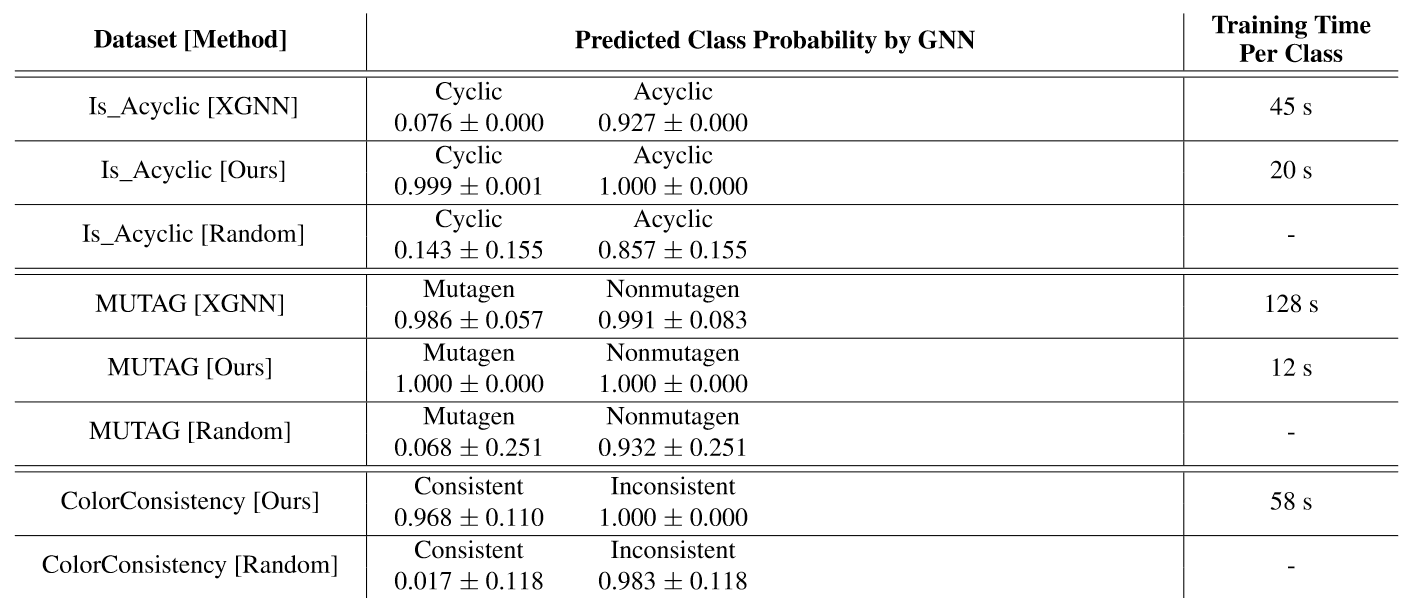
\includegraphics{figures/random_baseline.png} (Wang and Shen 2024)
  \end{itemize}

  For example, random graphs have an average predicted probability of
  being Non-mutagenic in the MUTAG dataset if 93.2\%. This demonstrates
  why the above objective is insufficient to generate realistic or
  \emph{in-distribution} (id) graph.

  \begin{itemize}
  \tightlist
  \item
    In order to mitigate this issue, the author proposed additional
    minimizing the cosine distance between the average embedding of all
    the observed graph from the targeted class, \(\bar h^{(L)}_{G_c}\),
    and the embedding of the generated explanation.
  \end{itemize}

  \begin{equation}
       \mathcal{L}_{\text{embed}}(\Theta \ | \ G_\text{gen}) = \text{CosDist}\left( \bar h^{(L)}_{G_c}, \ h^{(L)}_{G_\text{gen}} \right)
    \end{equation}
\item
  Regularization terms.

  \begin{itemize}
  \tightlist
  \item
    Sparse graphs are easy for humans to interpret. To encourage
    sparsity the authors employed an \(L_1\), \(L_2\), and a budget
    penalty on the edge probabilities.
  \end{itemize}

  \begin{equation}
        \mathcal{L}_{\text{Sparsity}}(\theta_A) = ||\theta_A||_1 + ||\theta_A||_2 + \text{softplus}(\text{sigmoid}||\theta_A||_1 - B)^2
    \end{equation} where \(B\) is the expected maximum number of edge
  for generated explanation graphs.

  \begin{itemize}
  \tightlist
  \item
    Connectivity is another desirable property as it ensures a cohesive
    explanation. To encourage connectivity the author minimize the
    \emph{KL-Divergence} between edge probabilities that share a common
    node.
  \end{itemize}

  \begin{equation}
        \mathcal{L}_{\text{Connect}}(\theta_A) = \sum_{i \in \nu} \sum_{j, k \in \mathcal{E}(i)} D_{KL}(\text{sigmoid}(\theta_A[i, \ j]) \ || \ \text{sigmoid}(\theta_A[i, \ k]))
    \end{equation}

  where \(\mathcal{E}(i)\) is the set of edges that connect to node
  \(i\).
\item
  Summary of Results + Figures

  \begin{itemize}
  \tightlist
  \item
    The final generator model is trained by sampling
    \(G_\text{gen} \sim \text{gen}(\Theta)\) and then iterative updated
    \(\Theta\) via gradient descent on the full loss: \begin{equation}
      \begin{split}
          \mathcal{L}_{\text{GNNInterpreter}}(\Theta \ | \ G_\text{gen}) = 
          &\mathcal{L}_{\text{pred}}(\Theta \ | \ G_\text{gen}) + 
          \mathcal{L}_{\text{embed}}(\Theta \ | \ G_\text{gen}) +  \\
          &\mathcal{L}_{\text{sparsity}}(\Theta \ | \ G_\text{gen}) +
          \mathcal{L}_{\text{connect}}(\Theta \ | \ G_\text{gen}) 
      \end{split}
      \end{equation}
  \end{itemize}

  \begin{figure}

  {\centering 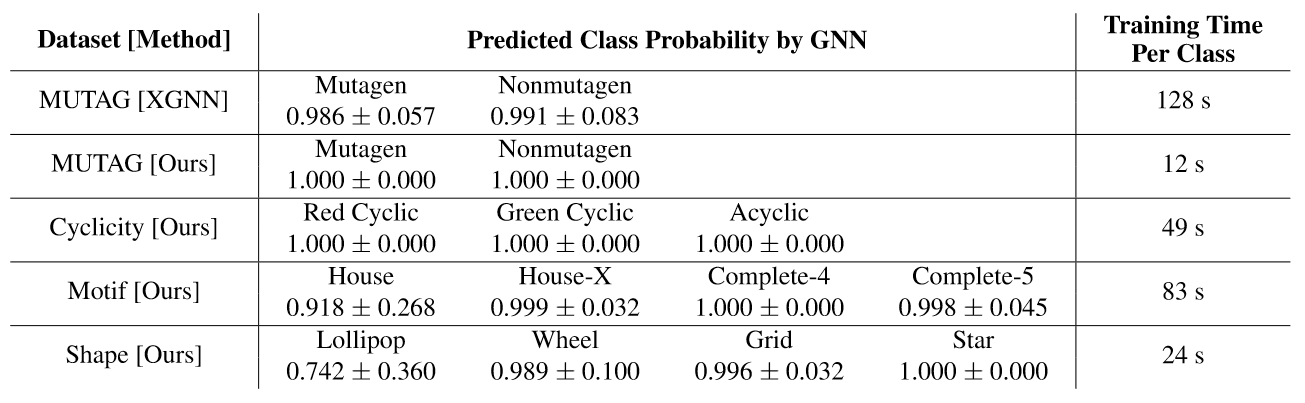
\includegraphics{figures/GNNInt_prediction_results.png}

  }

  \end{figure}

  \begin{itemize}
  \tightlist
  \item
    GNNInterpreter achieve remarkable accuracy on most target classes.
    Many of the interval are tight and very close to 1, which implies
    that the examples generated are almost always classified as the
    targeted class. The explanations for the house motif and the
    lollipop shape are worse in terms of predictions. Although the
    author critique the use of predictions as the sole objective, they
    do not use any other quantitative metric to evaluate the validity of
    their explanations.
  \end{itemize}

  \begin{figure}

  {\centering 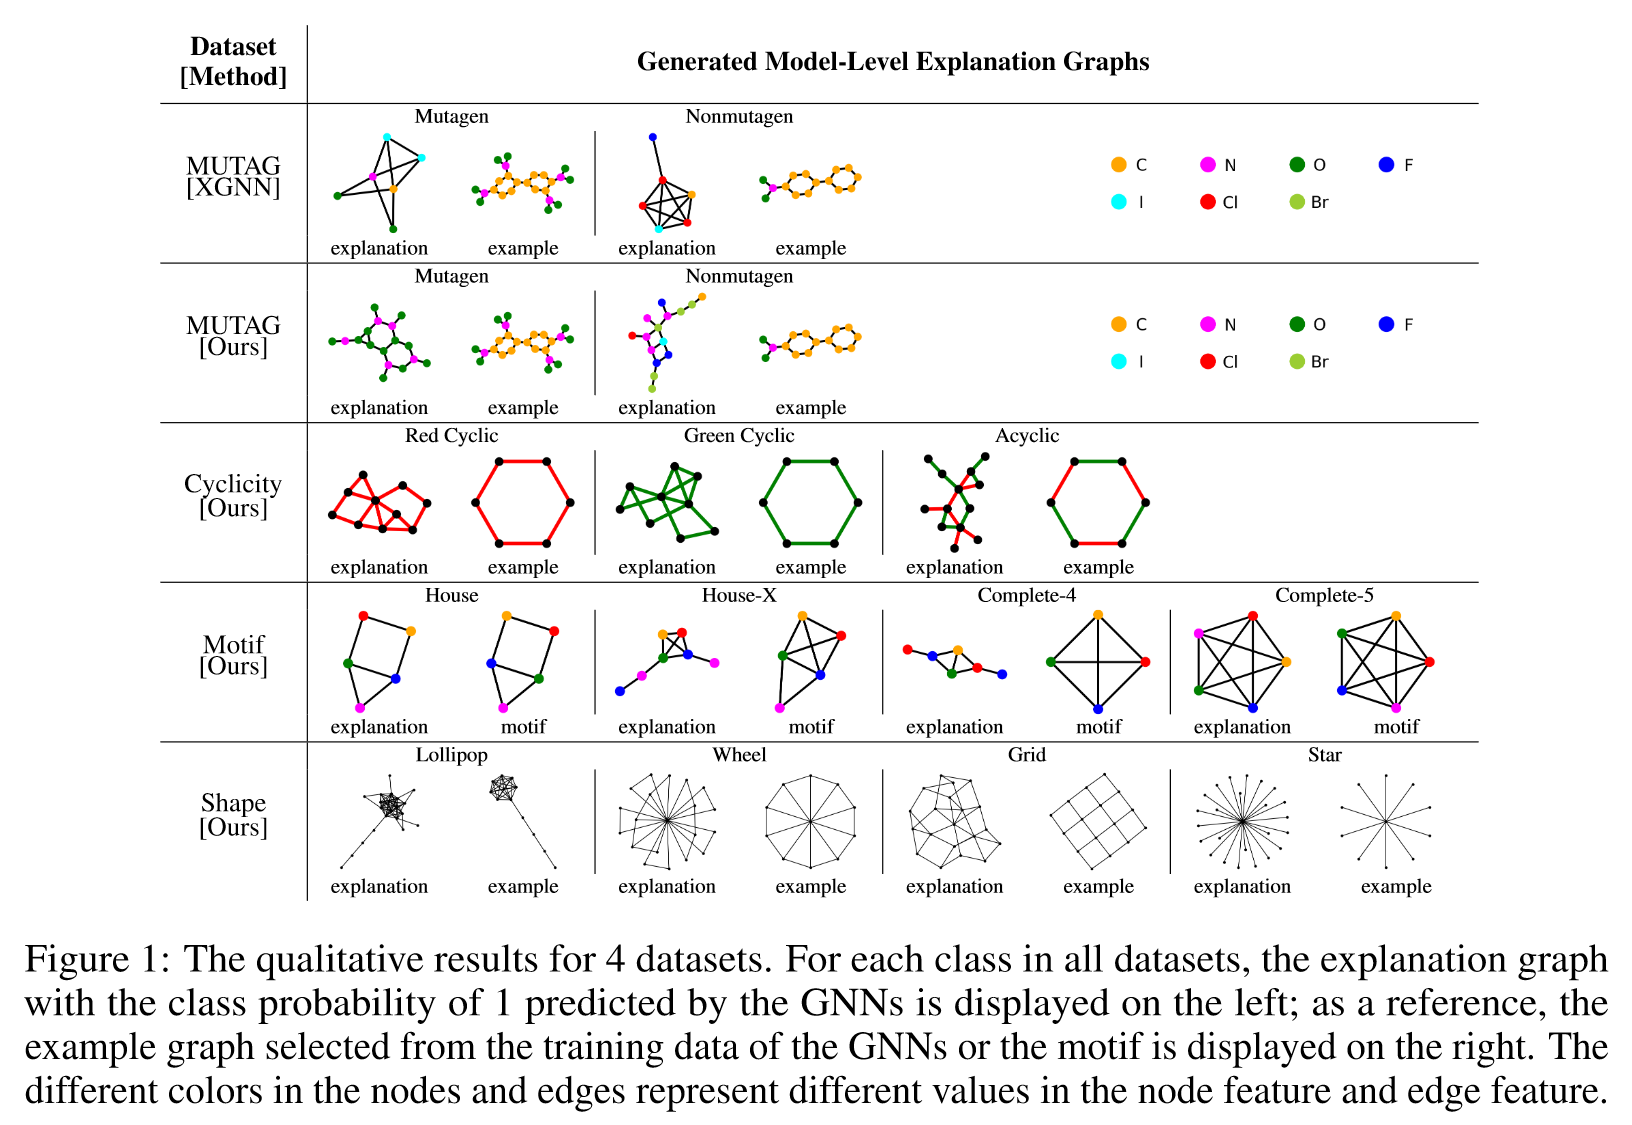
\includegraphics{figures/GNNInt_drawn_results.png}

  }

  \end{figure}

  \begin{itemize}
  \item
    Qualitatively we can see some limitation in terms of realism.
  \item
    For example, for the mutagen class, the explanation correctly
    identifies the importance of the N02 group; however, the generated
    graph isn't realistic and might not even be chemically possible.
    Furthermore, the non-mutagen example doesn't display any clear
    patterns or identifiable structures.
  \item
    The explanations for the Cyclicity dataset as well as the Wheel
    class do not appear to be members of the underlying data
    distribution.
  \item
    GNNInterpreter provides a way of generating example graph that would
    be classified as a target class by a GNN model, without needing to
    specify domain specific rules. On the other hand, optimizing
    predictions and even embeddings does not appear to be a sufficient
    objective for producing in-distribution graphs. The author correctly
    point out that optimizing predictions can lead to unrealistic
    graphs, but they have also inadvertently demonstrated that
    optimizing embeddings is not necessarily sufficient either.
  \end{itemize}
\end{itemize}

\hypertarget{d4explainer}{%
\subsection{D4Explainer}\label{d4explainer}}

(Chen et al. 2023)

\begin{itemize}
\item
  Overview

  \begin{itemize}
  \tightlist
  \item
    D4Explainer or in-Distribution GNN explanations via Discrete
    Denoising Diffusion attempt to directly address the realism of
    generated graphs in model-level explanation by using the observed
    data to train a Diffusion model.
  \item
    In the image domain, diffusion model have been shown to produce the
    most realistic images when compared to other generative AI methods
    such as Generative Adversarial Networks (GANs).
  \item
    Diffusion model work by iteratively noising an observation until it
    is pure noise. Then a denoising model is trained to predict the
    noise added at any given time step. Then new observations can be
    generated by passing pure noise through the diffusion model in a
    process known as reverse sampling.
  \item
    Additional label information can be passed to generate observations
    with similar a label.
  \end{itemize}
\item
  Generation Scheme

  \begin{itemize}
  \tightlist
  \item
    The authors of D4Explainer generate example graph by noising and
    de-nosing the adjacency matrices of observed graphs.
  \item
    The process of iteratively adding noise is known as forward
    diffusion.
  \item
    Let \(t \in [0, T]\) denote the iterative steps.
  \item
    \(A_t\) denote
  \end{itemize}
\item
  Loss Dist
\item
  Loss CF
\item
  Model-level sampling algorithm
\item
  CF-ACC
\item
  Fidelity
\item
  Density
\item
  MMD
\item
  Summary of Results + Figures
\item
  Forward Diffusion

  \begin{itemize}
  \tightlist
  \item
    The process of iteratively adding noise is known as forward
    diffusion.
  \item
    Let \(X_0\) be a noise free observation.\\
  \item
    If \(X_0\) is continuous, Gaussian noise is most common.
  \item
    Noise is added based on fixed hyperparameter known as the variance
    schedule and is denoted by \((\beta_1, \ \dots, \ \beta_T)\) where
    \(T\) is the total number of noising steps (theoretical \(X_T\) need
    to be pure noise).
  \item
    Using Gaussian noise, continuous forward diffusion is defined as
  \end{itemize}
\item
  Note on counter-factual explanations.
\end{itemize}

\hypertarget{protgnn}{%
\subsection{ProtGNN}\label{protgnn}}

(Zhang et al. 2021)

\hypertarget{synthesis-of-core-papers}{%
\section{Synthesis of Core Papers}\label{synthesis-of-core-papers}}

\begin{itemize}
\tightlist
\item
  Comparison of generation methods.

  \begin{itemize}
  \tightlist
  \item
    GNNInterpreter uses continuously relaxed discrete distributions.
  \item
    D4Explainer uses diffusion.
  \item
    Diffusion is slower, but can be more realistic. Probably because
    diffusion is less subject to the \textbf{out-of-distribution (OOD)
    problem}.
  \item
    Prototype projection are like generative methods. Restricted to in
    distribution, but realism is all but guaranteed.
  \end{itemize}
\end{itemize}

\hypertarget{technical-details}{%
\section{Technical Details}\label{technical-details}}

\begin{longtable}[t]{llllll}
\caption{}\\
\toprule
  & Predictions & Density & Deg. & CLus. & Spec.\\
\midrule
\addlinespace[0.3em]
\multicolumn{6}{l}{\textbf{GNNInterpreter Original}}\\
\hspace{1em}Class 0 & 1.0 +/- 0.0 & NA & NA & NA & NA\\
\hspace{1em}Class 1 & 1.0 +/- 0.0 & NA & NA & NA & NA\\
\addlinespace[0.3em]
\multicolumn{6}{l}{\textbf{GNNInterpreter Reimplemented}}\\
\hspace{1em}Class 0 & 0.93 +/- 0.01 & 0.38 +/- 0.002 & 1.77 & 1.53 & 0.07\\
\hspace{1em}Class 1 & 0.98 +/- 0.01 & 0.32 +/- 0.003 & 1.41 & 1.43 & 0.04\\
\addlinespace[0.3em]
\multicolumn{6}{l}{\textbf{D4Explainer Original}}\\
\hspace{1em}Aggregated & 0.92 & 0.315 & 0.12 & 0.00 & 0.02\\
\addlinespace[0.3em]
\multicolumn{6}{l}{\textbf{D4Explainer Reimplemented}}\\
\hspace{1em}Class 0 & 0.63 +/- 0.23 & 0.13 +/- 0.03 & 0.27 & 0.57 & 0.05\\
\hspace{1em}Class 1 & 0.66 +/- 0.20 & 0.13 +/- 0.03 & 0.08 & 0.25 & 0.04\\
\bottomrule
\multicolumn{6}{l}{\rule{0pt}{1em}\textsuperscript{1} +/- 1 standard deviation; 1000 graphs.}\\
\multicolumn{6}{l}{\rule{0pt}{1em}\textsuperscript{*} Empty}\\
\end{longtable}

\hypertarget{future-directions}{%
\section{Future Directions}\label{future-directions}}

\pagebreak

\hypertarget{references}{%
\section*{References}\label{references}}
\addcontentsline{toc}{section}{References}

\hypertarget{refs}{}
\begin{CSLReferences}{1}{0}
\leavevmode\vadjust pre{\hypertarget{ref-bai2019unsupervised}{}}%
Bai, Yunsheng, Hao Ding, Yang Qiao, Agustin Marinovic, Ken Gu, Ting
Chen, Yizhou Sun, and Wei Wang. 2019. {``Unsupervised Inductive
Graph-Level Representation Learning via Graph-Graph Proximity.''}
\url{https://arxiv.org/abs/1904.01098}.

\leavevmode\vadjust pre{\hypertarget{ref-Chen_Wu_Gupta_Ying_2023}{}}%
Chen, Jialin, Shirley Wu, Abhijit Gupta, and Rex Ying. 2023.
{``D4Explainer: In-Distribution GNN Explanations via Discrete Denoising
Diffusion,''} no. arXiv:2310.19321 (October).
\url{https://doi.org/10.48550/arXiv.2310.19321}.

\leavevmode\vadjust pre{\hypertarget{ref-gallicchio2019fast}{}}%
Gallicchio, Claudio, and Alessio Micheli. 2019. {``Fast and Deep Graph
Neural Networks.''} \url{https://arxiv.org/abs/1911.08941}.

\leavevmode\vadjust pre{\hypertarget{ref-Huijben_Kool_Paulus_van_Sloun_2022}{}}%
Huijben, Iris A. M., Wouter Kool, Max B. Paulus, and Ruud J. G. van
Sloun. 2022. {``A Review of the Gumbel-Max Trick and Its Extensions for
Discrete Stochasticity in Machine Learning,''} no. arXiv:2110.01515
(March). \url{https://doi.org/10.48550/arXiv.2110.01515}.

\leavevmode\vadjust pre{\hypertarget{ref-Maddison_Mnih_Teh_2017}{}}%
Maddison, Chris J., Andriy Mnih, and Yee Whye Teh. 2017. {``The Concrete
Distribution: A Continuous Relaxation of Discrete Random Variables,''}
no. arXiv:1611.00712 (March).
\url{https://doi.org/10.48550/arXiv.1611.00712}.

\leavevmode\vadjust pre{\hypertarget{ref-Wang_Shen_2024}{}}%
Wang, Xiaoqi, and Han-Wei Shen. 2024. {``GNNInterpreter: A Probabilistic
Generative Model-Level Explanation for Graph Neural Networks,''} no.
arXiv:2209.07924 (February).
\url{https://doi.org/10.48550/arXiv.2209.07924}.

\leavevmode\vadjust pre{\hypertarget{ref-Xiao_Wang_Rong_Yang_Zhang_Zhan_Bishop_Wilhelm_Zhang_Pickering_et_al._2023}{}}%
Xiao, Guanghua, Shidan Wang, Ruichen Rong, Donghan Yang, Xinyi Zhang,
Xiaowei Zhan, Justin Bishop, et al. 2023. \emph{Deep Learning of Cell
Spatial Organizations Identifies Clinically Relevant Insights in Tissue
Images}. Preprint. In Review.
\url{https://doi.org/10.21203/rs.3.rs-2928838/v1}.

\leavevmode\vadjust pre{\hypertarget{ref-Yuan_Yu_Gui_Ji_2022}{}}%
Yuan, Hao, Haiyang Yu, Shurui Gui, and Shuiwang Ji. 2022.
{``Explainability in Graph Neural Networks: A Taxonomic Survey,''} no.
arXiv:2012.15445 (July).
\url{https://doi.org/10.48550/arXiv.2012.15445}.

\leavevmode\vadjust pre{\hypertarget{ref-Zhang_Liu_Wang_Lu_Lee_2021}{}}%
Zhang, Zaixi, Qi Liu, Hao Wang, Chengqiang Lu, and Cheekong Lee. 2021.
{``ProtGNN: Towards Self-Explaining Graph Neural Networks,''} no.
arXiv:2112.00911 (December).
\url{https://doi.org/10.48550/arXiv.2112.00911}.

\end{CSLReferences}



\end{document}
